\documentclass[12pt]{article}

\usepackage[english, russian]{babel}
\usepackage[T2A]{fontenc}
\usepackage[utf8]{inputenc}
\usepackage[left=2cm,right=2cm, top=1cm,bottom=1.5cm,bindingoffset=0cm]{geometry}
\usepackage[explicit]{titlesec}
\usepackage{amsmath}
\usepackage{multirow}
\usepackage{bookmark}
\usepackage{minted}
\usepackage{hyperref}

\usepackage{graphicx}
\graphicspath{{images/}}
\DeclareGraphicsExtensions{.pdf,.png,.jpg}

\newcommand{\eref}[1]{\hyperref[{e:#1}]{\nameref*{e:#1} \ref*{e:#1}}}

\begin{document}
    \pagestyle{empty}
    \begin{center}
        \textbf{Федеральное государственное автономное образовательное учреждение высшего образования}

        \vspace{5pt}

        {\small
        \textbf{САНКТ-ПЕТЕРБУРГСКИЙ НАЦИОНАЛЬНЫЙ}

        \textbf{ИССЛЕДОВАТЕЛЬСКИЙ УНИВЕРСИТЕТ ИТМО}

        \textbf{ФАКУЛЬТЕТ ПРОГРАММНОЙ ИНЖЕНЕРИИ И КОМПЬЮТЕРНОЙ ТЕХНИКИ}%
        }

        \vspace{140pt}

        {\Large
        \textbf{ЗАДАНИЕ}

        \vspace{7pt}

        \textbf{ПО ДИСЦИПЛИНЕ}%
        }

        \vspace{10pt}

        {\large
        \textbf{Правовые основы интеллектуальной собственности}

        \vspace{5pt}

        \textbf{«Патентный поиск»}%
        }

        \vspace{170pt}

        \begin{tabular}{lll}
            Проверил:                                                                               & \hspace{70pt} & Выполнил:                                            \\
            ........................                \rule[0.66\baselineskip]{2cm}{0.4pt}                            &               & Студент группы P3555                                 \\
            «\rule[0.66\baselineskip]{1cm}{0.4pt}»  \rule[0.66\baselineskip]{2cm}{0.4pt} \the\year г.   &               & Федюкович С. А. \rule[0.66\baselineskip]{2cm}{0.4pt}  \\
            &               &                                                      \\
            Оценка          \hspace{12pt}           \rule[0.66\baselineskip]{2.7cm}{0.4pt}                               &               &                                                      \\
        \end{tabular}

        \vspace*{\fill}

        Санкт-Петербург

        \the\year
    \end{center}

    \newpage
    \pagestyle{plain}
    \setcounter{page}{1}

    \newpage
    \tableofcontents

    \newpage
    \section{Введение}

    Для проведения патентного поиска была выбрана область психологического тестирования в сфере информационных технологий.
    Перед проведением поиска был отобран список уже существующих организаций и продуктов в данной области:

    \begin{enumerate}
        \item CogniFit Inc --- Международная компания, которая работает в секторе цифрового здоровья и ориентирована на оценку и улучшение когнитивного здоровья.
        Более 3 миллионов пользователей.
        \item MorphCast --- Платформа для оценки эмоций пользователей с использованием технологий машинного обучения.
        Принадлежит компании Cynny S.p.A, состоящей внутри крупнейшей итальянской сети KPMG.
        Данных о количестве пользователей не предоставлено.
        \item SightCorp --- Компания по разработке программного обеспечения в Амстердаме, Нидерланды.
        Специализируется на автоматичческом определении движений мимики лица, настроения и поведения.
        Данных о количестве пользователей не предоставлено.
    \end{enumerate}

    \newpage

    \section{Поиск патентов}

    \subsection{Компания CogniFit}

    Проведём поиск по компании CogniFit, так как компания является международной, то достаточно будет провести поиск по базе данных Европейского патентного ведомства:

    \begin{figure}[ht]
        \centering
        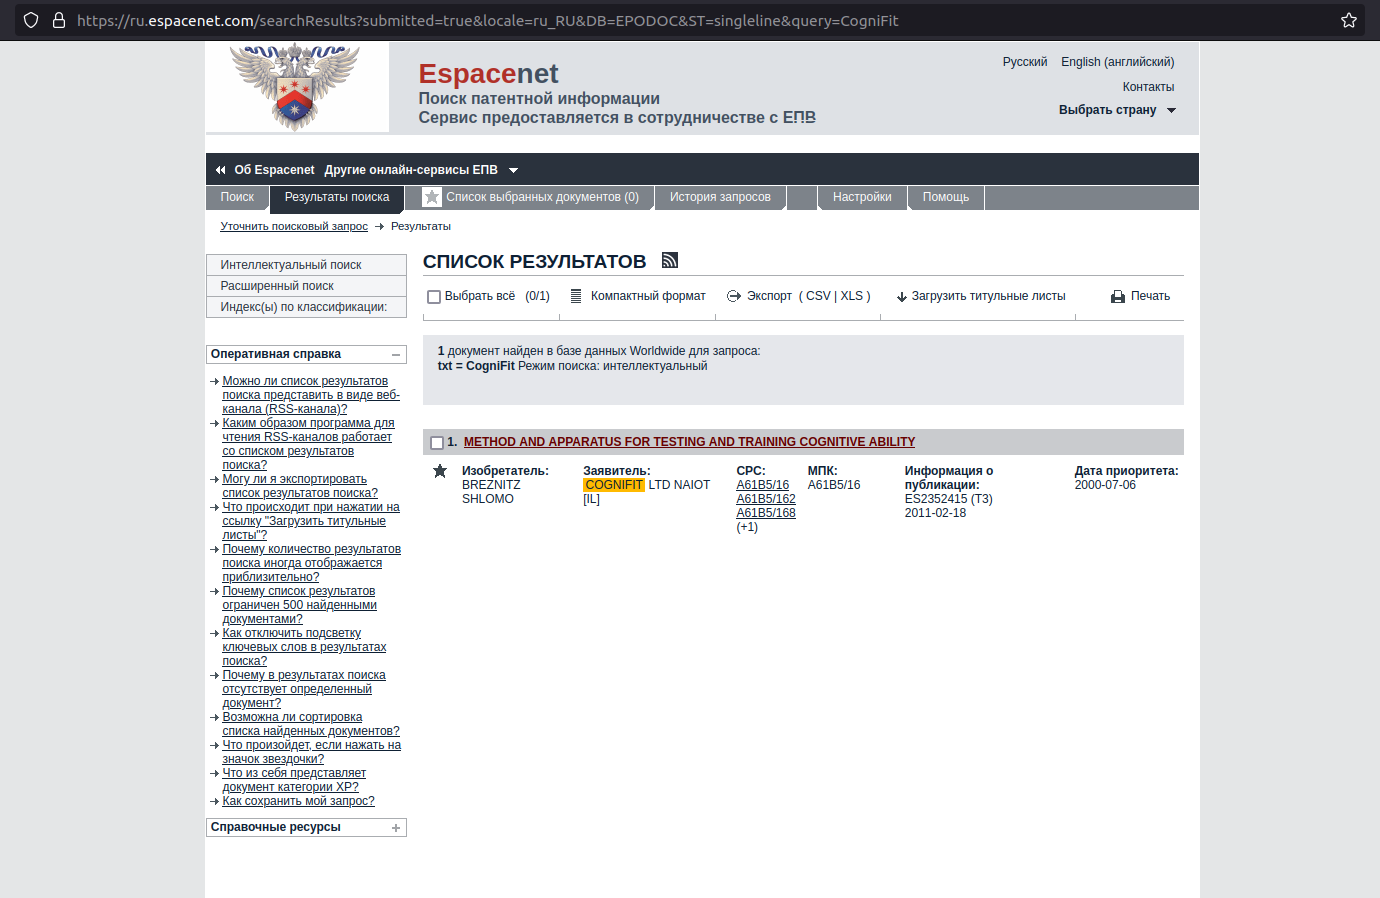
\includegraphics[scale=1.5]{images/1.png}
        \caption{Патенты компании CogniFit}
        \label{fig:o:1}
    \end{figure}

    Среди патентов был найден ровно один: \href{https://ru.espacenet.com/publicationDetails/biblio?FT=D&date=20110218&DB=EPODOC&locale=ru_RU&CC=ES&NR=2352415T3&KC=T3&ND=5}{METHOD AND APPARATUS FOR TESTING AND TRAINING COGNITIVE ABILITY}.

    Исходный текст патента:

    A method for testing and/or training cognitive ability, including the steps of testing a preliminary cognitive level of a user and receiving results representative therefrom.
    According to the results, the cognitive level may then be broken up into separate discrete cognitive skills, and one or more tasks may be created, each task related to each of the separate discrete cognitive skills.
    The one or more tasks may then be presented to the user and so that a current cognitive level of the user is re-tested, and results representative therefrom are received.
    This process may be repeated at least one time.;A method for testing and/or training cognitive ability (step 10 - step 506), including the steps of testing a preliminary cognitive level of a user (step 10) and receiving results representative therefrom (step 12).
    According to the results, the cognitive level may then be broken up into separate discrete cognitive skills (step 14), and one or more tasks may then be created (step 18), each task related to each of the discrete cognitive skills.
    The one or more tasks may then be presented to the user and so that a current cognitive level (step 20) of the user is re-tested, and results representative therefrom are received.
    This process may be repeated at least one time (step 408).

    \begin{figure}[ht]
        \centering
        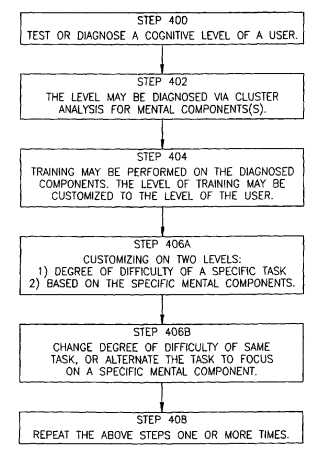
\includegraphics[scale=0.8]{images/2.png}
        \caption{Титульный лист патента METHOD AND APPARATUS FOR TESTING AND TRAINING COGNITIVE ABILITY}
        \label{fig:o:2}
    \end{figure}

    Данный патент является патентом на полезную модель, описывающий проведение тестов на определение когнитивных навыков и последующую их тренировку на основании этих данных.
    Срок действия патента закончился в 2020 году, поэтому данный патент представляет только исторический интерес о деятельности компании CogniFit в период с 2000ые по 2020ые годы.

    \subsection{Компания Cynny SPA}

    Проведём поиск аналогично предыдущей компании, поскольку Cynny SPA так же является международной:

    \begin{figure}[ht]
        \centering
        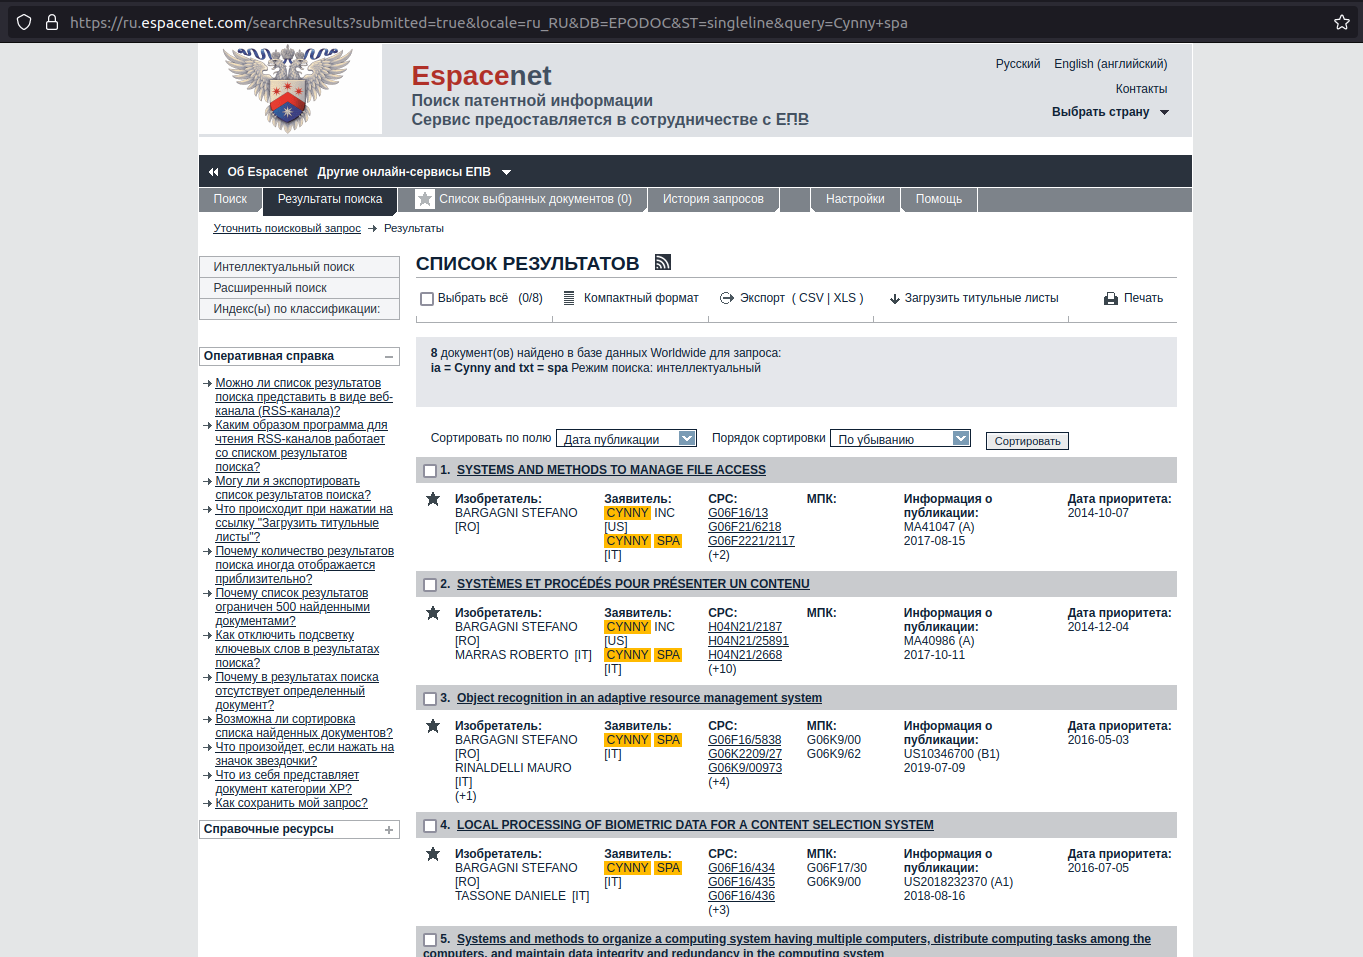
\includegraphics[scale=1.5]{images/3.png}
        \caption{Патенты компании Cynny SPA}
        \label{fig:o:3}
    \end{figure}

    Были найден следующий список патентов:

    \begin{enumerate}
        \item SYSTEMS AND METHODS TO MANAGE FILE ACCESS
        \item SYSTÈMES ET PROCÉDÉS POUR PRÉSENTER UN CONTENU
        \item Object recognition in an adaptive resource management system
        \item LOCAL PROCESSING OF BIOMETRIC DATA FOR A CONTENT SELECTION SYSTEM
        \item Systems and methods to organize a computing system having multiple computers, distribute computing tasks among the computers, and maintain data integrity and redundancy in the computing system
        \item SYSTEMS AND METHODS TO PRESENT CONTENT
        \item SYSTEMS AND METHODS TO PRESENT CONTENT
        \item SYSTEMS AND METHODS TO ORGANIZE A COMPUTING SYSTEM HAVING MULTIPLE COMPUTERS, DISTRIBUTE COMPUTING TASKS AMONG THE COMPUTERS, AND MAINTAIN DATA INTEGRITY AND REDUNDANCY IN THE COMPUTING SYSTEM
    \end{enumerate}

    Среди данных патентов под искомую область подходит только \href{https://ru.espacenet.com/publicationDetails/biblio?DB=EPODOC&II=3&ND=3&adjacent=true&locale=ru_RU&FT=D&date=20180816&CC=US&NR=2018232370A1&KC=A1#}{LOCAL PROCESSING OF BIOMETRIC DATA FOR A CONTENT SELECTION SYSTEM}

    Исходный текст патента:

    A data processing method implemented on a computing device, the method including: capturing, using a camera, an image during playback of recommendation determination content, where the recommendation determination content is used by the computing device to present customized content in response to the recommendation determination content;
    determining, based on the image that was captured, biometric information of a subject in the captured image;
    determining an object category of the recommendation determination content played on the computing device;
    storing, locally on the computing device, a profile associating the biometric information and the object category of the recommendation determination content, based on using the biometric information to identify the profile from another profile stored on the computing device; determining, based on the profile stored on the computing device, a predetermined content access category, where the predetermined content access category represents a type of content that may be of interest when played at the computing device; causing, based on the predetermined content access category and without the biometric information that was used to generate the predetermined content access category, selection of customized content for display on the computing device.

    \begin{figure}[ht]
        \centering
        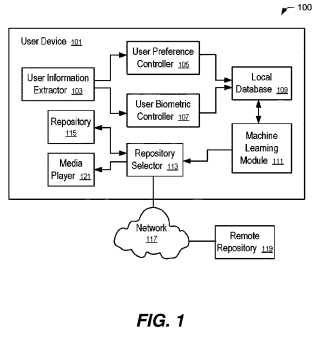
\includegraphics[scale=0.8]{images/4.png}
        \caption{Титульный лист патента LOCAL PROCESSING OF BIOMETRIC DATA FOR A CONTENT SELECTION SYSTEM}
        \label{fig:o:4}
    \end{figure}

    Данный патент так же, как и предыдущий, является патентом на полезную модель, описывающий сбор биометрических данных, их обработку при помощи машинного обучения, а так же хранения и использования этих данных в целях использования в системах рекомендации контента.
    Рассмотрение патента было приостановлено в 2018 году, поэтому данный патент так же предоставляет только исторический интерес о возможной деятельности компании Cynny SPA в период с 2016ый по 2018ый года.

    \subsection{Компания Sightcorp}

    Проведём аналогичный поиск:

    \begin{figure}[ht]
        \centering
        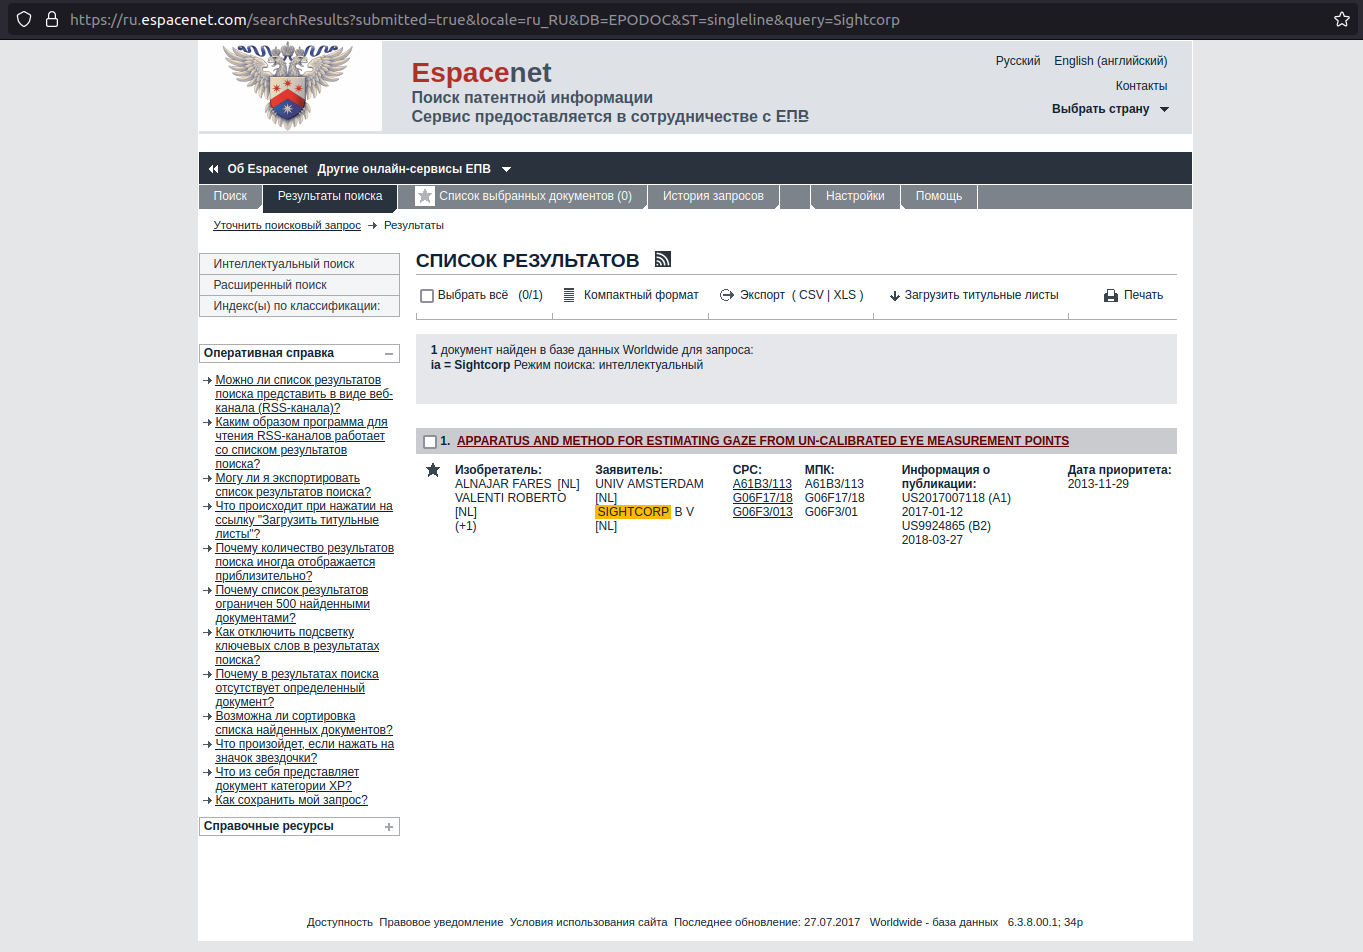
\includegraphics[scale=1.5]{images/5.png}
        \caption{Патенты компании Sightcorp}
        \label{fig:o:5}
    \end{figure}

    Среди патентов был найден ровно один: \href{https://ru.espacenet.com/publicationDetails/biblio?DB=EPODOC&II=0&ND=3&adjacent=true&locale=ru_RU&FT=D&date=20170112&CC=US&NR=2017007118A1&KC=A1#}{APPARATUS AND METHOD FOR ESTIMATING GAZE FROM UN-CALIBRATED EYE MEASUREMENT POINTS}.

    Исходный текст патента:

    Some embodiments are directed to a system and a method for estimating gaze from a set of eye measurement points that are indicative of a gaze pattern of a user viewing a scene.
    Some other embodiments are directed to obtaining sets of eye measurement points from different users viewing the same scene.
    In another embodiment, the different sets of eye measurement points are mapped to a common coordinate system for reciprocal calibration.
    In yet another embodiment, a scene transformation for mapping the common coordinate system to a coordinate system associated with the scene can be calculated by matching eye measurement points from the common coordinate system to interest points of the scene.
    The scene transformation is thereby calculated more accurately than individually calculated scene transformations, thereby providing a more accurate estimate of the gaze points.

    \begin{figure}[ht]
        \centering
        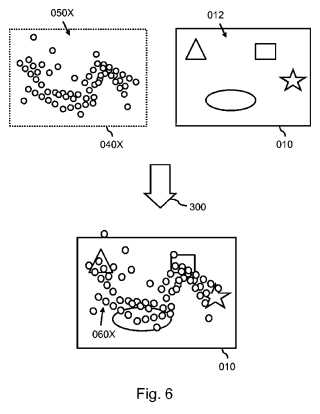
\includegraphics[scale=0.8]{images/6.png}
        \caption{Титульный лист патента APPARATUS AND METHOD FOR ESTIMATING GAZE FROM UN-CALIBRATED EYE MEASUREMENT POINTS}
        \label{fig:o:6}
    \end{figure}

    Данный патент так же, как и предыдущий, является патентом на полезную модель, описывающий способ отслеживания движения глаз при помощи программно-аппаратных средств.
    В данное время патент активен и его действие по плану должно закончиться в 2034 году. Отсюда следует, что данная компания, скорее всего, ведёт активную разработку и продвижение данного решения.

    \newpage

    \section{Список источников}

    \begin{enumerate}
        \item \href{https://www.cognifit.com/ru/whats-cognifit}{https://www.cognifit.com/ru/whats-cognifit} --- Что такое CogniFit ("КогниФит")?
        \item \href{https://www.morphcast.com/societa}{https://www.morphcast.com/societa} --- Cynny S.p.A MorphCast (на итальянском языке).
        \item \href{https://sightcorp.com/about-us/}{https://sightcorp.com/about-us/} --- About Sightcorp (на английском языке).
    \end{enumerate}
\end{document}